\section{Codificação}

\begin{frame}[allowframebreaks]
  \frametitle{Codificação}
  \begin{itemize}
  \item Codificação sem perdas de informação de fontes regidas por uma determinada distribuição.
  \item Teorema da Codificação de Shannon: é possível codificar utilizando $R > H(X)$ bits por
	símbolo da fonte, se utilizarmos bloco grande suficiente.
  \item Transmissão de blocos não é prática.
  \item Outras alternativas:
	\begin{enumerate}
	\item Códigos de tamanho variável: os símbolos são codificados separadamente utilizando
		palavras de código com comprimento variável. Ex: Codificação Huffman.
	\item Codificação de Fluxo (\textit{stream code}): codificação que opera no fluxo de dados,
		decidindo a palavra código dependendo do símbolo corrente e da história 
		(símbolos passados). Ex: Codificação Aritmética, Codificação Lempel-Ziv
		(sendo este ultimo um codificação universal, pois não requer $p(x)$).
	\end{enumerate}
  \item Queremos uma codificação prática que alcance o limite da entropia.
  \item A codificação pode utilizar a distribuição $p(x)$ dada, ou estimá-la de alguma forma.
  \item Não iremos lidar aqui com o problema de estimar $p(x)$ (problema de estimação de densidade),
	vamos supor que $p(x)$ é conhecido ou sua aproximação $q(x)$ é dada.
  \item Vamos verificar o efeito de utilizar a aproximação $q(x)$ quando a distribuição subjacente é $p(x)$.
  \end{itemize}
\end{frame}

\begin{frame}[allowframebreaks]
  \frametitle{Codificação de Fonte}
  \begin{definition}[Codificação de Fonte]
  Um código $C$ para a v.a. $X$ é um mapeamento de $\mathcal{X}$ em $\mathcal{D}^\ast$, 
  ou seja 
	\begin{equation} 
	C: \mathcal{X} \rightarrow \mathcal{D}^\ast , 
	\end{equation} 
  onde $\mathcal{D}^\ast$ é o conjunto
  de sequências (\textit{strings}) finitas em um alfabeto $D$-ário. $C(x)$ é a palavra código 
  (\textit{codeword}) correspondente ao símbolo $x$, e $l(x)$ é o comprimento desta palavra.
  \end{definition}

  \begin{example}
  Seja $\mathcal{X} = \{\text{azul}, \text{vermelho}\}$. O código pode ser $C(\text{vermelho})=00$ e 
  $C(\text{azul})=11$, o que seria um código binário para $\mathcal{D} = \{0,1\}$.
  Teríamos então $\mathcal{D}^\ast = \{ 00 , 11 \}$. Uma sequência produzida pela fonte da forma
  $(\text{azul},\text{azul},\text{vermelho})$ seria codificada como $(11,11,00)$, ou melhor, $111100$.
  \end{example}

  \framebreak

  \begin{definition}[Comprimento Esperado]
  O comprimento esperado $L(C)$ de um código $C$ para uma v.a. $X$ com distribuição $p(x)$ é dado por
	\begin{equation}
	L(C) = \sum_x p(x) l(x)
	\end{equation}
  \end{definition}

  \framebreak

  \begin{itemize}
  \item De forma geral, $\mathcal{D} = \{0,1, \ldots, D-1\}$, mas usualmente utilizamos $D=2$.
  \end{itemize}
  \begin{example}
     \begin{columns}
     \begin{column}{0.45\textwidth}
	Seja $\mathcal{X} = \{1, 2, 3, 4\}$ e $\mathcal{D} = \{0, 1\}$. Podemos definir 
	o código através da tabela.
     \end{column}
     \begin{column}{0.45\textwidth}
	\begin{tabular}{c|c|c|c}
	x & p(x)  & c(x) & l(x) \\ \hline
	1 & $1/2$ & 0    & 1	\\
	2 & $1/4$ & 10   & 2	\\
	3 & $1/8$ & 110  & 3	\\
	4 & $1/8$ & 111  & 3	\\
	\end{tabular}
     \end{column}
     \end{columns}
    \examplebreak
    \begin{itemize}
    \item Neste caso, teremos $H(X) = 1.75$ e $L(C)=El(X)=1.75$, então este código é muito bom.
    \item A decodificação para este código é fácil.
    \item Qual é a sequência de símbolos que produziu a seguinte sequência 010110111111110100? R: 1,2,3,4,4,3,2,1.
    \item Com pontuação separando os símbolos: 0,10,110,111,111,110,10,0. Dizemos que o código possui pontuação
	automática.
    \end{itemize}
  \end{example}

  \framebreak

  \begin{example}
  Vamos considerar $\mathcal{X} = \{1,2,3\}$ e $\mathcal{D}=\{0,1\}$.
 
  Código:
  \begin{tabular}{cccc}
  x      &  1    &   2   &   3   \\ \hline
  $p(x)$ & $1/3$ & $1/3$ & $1/3$ \\ \hline
  $C(X)$ & $0$   & $10$  & $11$  
  \end{tabular}

  Teremos então $H = 1.58$bits e $El(X)=1.66 > H$ bits.
  \end{example}

  Podemos facilmente decodificar? Por exemplo: $10110010 = 2,3,1,1,2$.


  \framebreak


  \begin{figure}[h!]
  \centering
  \includegraphics[width=0.4\textwidth]{images/International_Morse_Code.pdf}
  \label{fig:International_Morse_Code}
  \end{figure}

  \begin{itemize}
  \item Note que um código pode ser um prefixo de outro.
  \end{itemize}

  \framebreak

  Para $\mathcal{X} = \{1,2,3,4\}$ e $\mathcal{D}=\{0,1\}$ (código binário), considere os seguintes códigos

  \begin{center}
  \begin{tabular}{c|c|c|c|c|c}
  $x$ 		& $p(x)$& $C_I$ & $C_{II}$ & $C_{III}$ & $C_{IV}$ \\ \hline
  1		& 0.5	&  0	&   0	&  0 		&   0	\\ 
  2		& 0.25	&  0	&   1 	& 10		&  01	\\
  3		& 0.125	&  1	&  00	& 110		& 011 	\\
  4		& 0.125	& 10	&  11	& 111 		& 0111 	\\
  $H(X)$	& 1.75	&  -	&  -	&  -		&  -	\\
  $El(X)$ 	&  -	& 1.125	& 1.25	&  1.75		& 1.875
  \end{tabular}
  \end{center} 

  \begin{itemize}
  \item Eficiência do Código = $H(X) / El(X)$.
  \item Geralmente preferimos códigos com comprimento esperado menor.
  \item Note que o código $C_I$ não é unívoco. A sequência $00001$ pode ser decodificada como
	$1,2,1,2,3$ ou $2,1,2,1,3$ ou $1,1,1,1,3$ ...
  \item O valor esperado do comprimento do código não pode ser menor que a entropia sem que o código
	incorra em erro.
  \item Considere $C_{II}$. Qual seria o resultado da decodificação de $0011$? Poderia ser
	$,1,1,2,2$ ou $3,4$ ou $3,2,2$ ou $1,1,4$. Novamente, não é possível decodificar sem
	que a probabilidade de erro seja nula (quando a sequência torna-se mais longa, a probabilidade
	de erro tende a $1$).
  \item O código $C_{III}$ é factível (já que $El \geq H$). O processo de decodificação é simples.
	Por exemplo: $111110100 = 111,110,10,0 = 4,3,2,1$.
  \item Utilizando o código $C_{IV}$ é possível decodificar a sequência $00000000111$? Sim, mas 
	os símbolos não são instantaneamente decodificados, é necessário ver os bits à frente para 
	conseguir decodificar.
  \end{itemize}
 
\end{frame}



\subsection{Tipos de Código}
\begin{frame}[allowframebreaks]
  \frametitle{Tipos de Código}

  \begin{definition}[extensão]
  Um extensão $C^\ast$ de um código $C$ é um mapeamento de uma sequência finita 
  de símbolos em $\mathcal{X}$ em uma sequência finita de símbolos em $\mathcal{D}$ através da
  concatenação dos códigos: 
  	\begin{equation}
	C^\ast (x_1,x_2,\ldots,x_n) = C(x_1) C(x_2) \ldots C(x_n)
	\end{equation}
  \end{definition}
  \begin{example}
  Se $C(x_1)=0$ e $C(x_2)=1$, então $C(x_1,x_2) = 01$.
  \end{example}
  \begin{example}
  Se $C(x_1)=000$ e $C(x_2)=100$, então $C(x_1,x_2,x_2) = 000100100$.
  \end{example}

  \framebreak

  \begin{definition}[não-singular]
  Um código é dito \textbf{não-singular} se todo elemento de $\mathcal{X}$
  é mapeado em sequências (\textit{strings}) diferentes em $\mathcal{D}^\ast$. I.e.,
	\begin{equation}
	x_i \neq x_j \Rightarrow C(x_i) \neq C(x_j)
	\end{equation}
  \end{definition}

  \begin{figure}[h!]
  \centering
  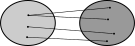
\includegraphics[width=0.5\textwidth]{images/nonsingularmap2.pdf}
  \label{fig:nonsingularmap}
  \end{figure}

  \framebreak

  \begin{definition}[decodificação unívoca]
  Um código $C$ com extensão $C^\ast$ é decodificável univocamente se a sua extensão $C^\ast$ for não-singular.
  \end{definition}
  
  \begin{itemize}
  \item Objetivo: transmitir ou armazenar uma sequência de símbolos na forma de uma sequência de palavras codificadas.
  \item Um código não-singular pode se tornar único se inserirmos pontuação, mas para isto seria necessário incluir
	um novo símbolo no alfabeto $\mathcal{D}$, o que aumentaria a taxa $R$.
  \item É preferível um código com característica de auto-pontuação e que seja instantâneo.
  \end{itemize}

  \framebreak

  Considere o código

  \begin{center}
  \begin{tabular}{ccccc}
  $x$    & 1  & 2  & 3  & 4 \\ \hline
  $C(x)$ & 10 & 00 & 11 & 110
  \end{tabular}
  \end{center}

  \begin{itemize}
  \item Este código é unicamente decodificável.
  \item Ex.: 1100000000 = 3,2,2,2,2.
  \item Ex.: 11000000000 = 4,2,2,2,2.
  \item Note que só sabemos a identidade do primeiro símbolo após ler toda a sequência.
  \end{itemize}

  \framebreak

  \begin{definition}[código de prefixo]
  Um código é chamado \textbf{código de prefixo} ou \textbf{código instantâneo} se nenhum palavra
  é prefixo de qualquer outra palavra.
  \end{definition}

  \begin{itemize}
  \item Quando temos um código de prefixo, sabemos onde está o fim de uma palavra, pois ela não
	é prefixo de nenhuma outra, ou seja, não existe nenhuma outra palavra que comece com a palavra
	encontrada.
  \item Um código de prefixo possui então a propriedade de auto-pontuação.
  \item Código de prefixo $\Rightarrow$ unicamente decodificável. 
	Mas unicamente decodificável $\nRightarrow$ código de prefixo.
  \end{itemize}
 
  \framebreak

  \begin{figure}[h!]
  \centering
  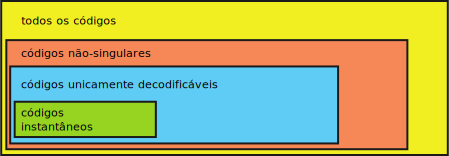
\includegraphics[width=0.75\textwidth]{images/tiposcodigos.pdf}
  \label{fig:tiposcodigos}
  \end{figure}

  \begin{itemize}
  \item Queremos um código com comprimento esperado mínimo possível.
  \item Analisando as classes de códigos, intuitivamente pensamos que é mais provável encontrarmos
	um código com comprimento esperado menor em uma classe maior (ou mais abrangente).
  \item Podemos alcançar um resultado melhor que a entropia se não utilizarmos um código não-singular,
	entretanto, queremos uma codificação sem perda.
  \end{itemize} 
\end{frame}



\subsection{Desigualdade de Kraft}
\begin{frame}[allowframebreaks]
  \frametitle{Desigualdade de Kraft}

  \begin{theorem}[Desigualdade de Kraft]
  Para qualquer código instantâneo (código de prefixo) sobre um alfabeto de tamanho $D$, o comprimento
  das palavras $l_1, l_2, \ldots, l_m$ deve satisfazer 
	\begin{equation}
	\sum_i D^{-l_i} \leq 1 .
	\end{equation}
  Por um outro lado, dado um conjunto de comprimentos de código satisfazendo a desigualdade acima,
  então existe um código de prefixo com estes comprimentos.
  \end{theorem}

  \begin{itemize}
  \item Note que foi dito que existe um código de prefixo com aqueles comprimentos, não significa que todos códigos
	cujos comprimentos satisfazem a desigualdade são códigos de prefixo.
  \item Se existe um código não-instantâneo com comprimentos $l_i$ satisfazendo a desigualdade de Kraft, então
	podemos encontrar um outro código, que terá a propriedade de prefixo, e que possuirá os mesmos comprimentos $l_i$,
	consequentemente não alterando o comprimento esperado.
  \item Logo, será sempre melhor escolher um código de prefixo.
  \end{itemize}

  \framebreak

  \begin{proof}[Desigualdade de Kraft]
  Vamos representar o conjunto de códigos em uma árvore $D$-ária (não necessariamente balanceada).

  \begin{figure}[h!]
  \centering
  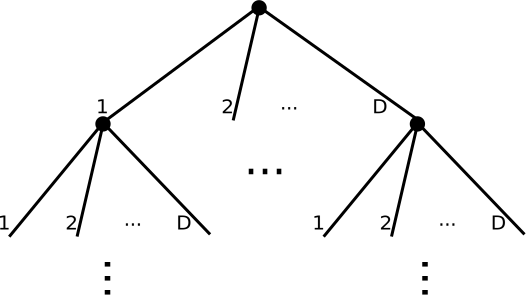
\includegraphics[width=0.5\textwidth]{images/Dtree.pdf}
  \label{fig:Dtree}
  \end{figure}
  
  \proofbreak

  \begin{itemize}
  \item As palavras correspondem à folhas na árvore.
  \item O caminho da raiz até a folha determina a palavra código.
  \item A condição de prefixo implica que não existe uma palavra a não ser nas folhas 
	(nenhum descendente de uma palavra código será também uma palavra código).
  \item $l_{\text{max}} = \max_i (l_i)$ é o comprimento da palavra mais longa.
  \item Podemos expandir toda a árvore até o comprimento $l_{\text{max}}$.
  \item Os nós no nível de $l_{\text{max}}$ são:
	\begin{enumerate}
	\item palavras de código;
	\item descendentes de palavras de código; ou
	\item nem um, nem outro.
	\end{enumerate}
  \end{itemize}
  \proofbreak
  \begin{itemize}
  \item Considere uma palavras $i$ no nível $l_i$ da árvore (então esta palavra possui comprimento $l_i$).
  \item Existem então $D^{l_{\text{max}} - l_i}$ descendentes de $i$, na árvore, no nível $l_{\text{max}}$.
  \item Com a condição de prefixo, podemos afirmar que os descendentes de código $i$ no nível $l_i$ são
	disjuntos dos descendentes do código $j$ no nível $l_j$, quando $i \neq j$ (i.e., o conjunto de
	descendentes para diferentes palavras é disjunto).
  \item O número total de nós em um conjunto de todos descendentes é $\leq D^{l_{\text{max}}}$.
  \end{itemize}
  \proofbreak
  \begin{itemize}
  \item Utilizando o que vimos acima, temos que a soma do número de descendentes de todos os códigos é menor ou
	igual ao número de folhas na árvore cheia no nível $l_{\text{max}}$. Podemos então escrever
	\begin{equation}
	\sum_i D^{l_{\text{max}} - l_i} \leq D^{l_{\text{max}}} \quad \Rightarrow \quad \sum_i D^{-l_i} \leq 1
	\end{equation}
  \item Por outro lado, dados os comprimentos $l_1, l_2, \ldots, l_m$, satisfazendo Kraft, iremos mostrar como
	construir um código de prefixo utilizando estes comprimentos.
  \item Considere uma árvore $D$-ária cheia de profundidade $l_{\text{max}}$ e $D^{l_{\text{max}}}$ nós terminais.
  \end{itemize}
  \proofbreak
  \begin{itemize}
  \item Observe que
	\begin{enumerate}
	\item No nível 0 existe uma fração $1$ de descendentes de cada nó neste nível;
	\item No nível 1 existe uma fração $1/D$ de descendentes de cada nó neste nível;
	\item No nível 2 existe uma fração $1/D^2$ de descendentes de cada nó neste nível;
	\item ...
	\end{enumerate}
  \item De forma geral, em cada nível $i \in [0, l_{\text{max}}]$ da árvore, existe uma fração de $D^{-i}$
	nós terminais que são descendentes de uma ramificação de cada um dos $D^i$ nós no nível $i$.
  \end{itemize}
  \proofbreak
  \begin{itemize}
  \item Ordene então os comprimentos $(l_1, l_2, \ldots, l_m)$ de forma ascendente $(s_1, s_2, \ldots, s_m)$, 
	sendo $s_1 \leq s_2 \leq \ldots \leq s_m$. Observe que existem tantos comprimentos quanto existem palavras.
  \item Para o comprimento $s_1$, escolha um nó no nível $s_1$ para indicar o código.
  \item Para garantir a condição de prefixo, o nó escolhido deve se tornar um nó terminal, eliminando assim uma
	fração $D^{-s_1}$ de nós terminais no nível $l_{\text{max}}$.
  \item Em seguida, escolha um dos nós remanescentes no nível $s_2$ (neste momento, existem $(D^{s_1}-1)D^{s_2-s_1}$
	possíveis escolhas), eliminando assim uma fração $D^{-s_2}$ de nós terminais no nível $l_{\text{max}}$.
  \end{itemize}
  \proofbreak
  \begin{itemize}
  \item A fração total de nós eliminados, até o momento, foi de $D^{-s_1} + D^{-s_2}$.
  \item Continuando este processo, iremos eliminar uma fração $\sum_{i=1}^{m} D^{-s_i}$ de nós, e neste processo
	estamos garantindo que estamos criando um código instantâneo (uma palavra de código não pode ser prefixo de outra).
  \item Como por suposição temos $\sum_{i=1}^{m} D^{-s_i} \leq 1$, nunca iremos eliminar mais do que todas as palavras
	de código, então este processo não irá exaurir as palavras de código.
  \item Criamos assim um código de prefixo com os comprimentos desejados, satisfazendo Kraft.
  \end{itemize}

  \end{proof}
\end{frame}


\begin{frame}[allowframebreaks]
  \frametitle{Kraft Infinito}

  \begin{theorem}[Kraft infinito contável]
  Para qualquer conjunto infinito contável de palavras de código que formam um conjunto com prefixo,
  este conjunto satisfaz a desigualdade de Kraft estendida, i.e.
	\begin{equation}
	\sum_{i=1}^{\infty} D^{-l_i} \leq 1
	\end{equation}
  Por outro lado, dados $l_i$s satisfazendo a equação acima, existe um código de prefixo com estes comprimentos.
  \end{theorem}

  \framebreak

  \begin{proof}[Kraft Infinito]
  \begin{itemize}
  \item Assuma que tenhamos um código de prefixo infinito contável e que o alfabeto é $D$-ário $\{0,1,\ldots,D-1\}$.
  \item Considere a $i$-ésima palavra $y_1,y_2,\ldots,y_{l_i}$.
  \item A expansão da $i$-ésima palavra, de comprimento $l_i$, utilizando os dígitos fracionários é da forma
	\begin{equation}
	0.y_1 y_2 y_3 \ldots y_{l_i} = \sum_{j=1}^{l_i} y_j D^{-j}
	\end{equation}
  \end{itemize}
  \proofbreak
  \begin{itemize}
  \item Considere os exemplos com $D=2$ e $\mathcal{D} = \{0,1\}$:
  	\begin{itemize}
	\item $0.1 = 1 \times 2^{-1} = \frac{1}{2}$
 	\item $0.01 = 0 \times 2^{-1} + 1 \times 2^{-2} = \frac{1}{4}$
	\item $0.11 = 1 \times 2^{-1} + 1 \times 2^{-2} = \frac{3}{4}$
	\item $0.001 = 1 \times 2^{-1} + 1 \times 2^{-2} + 1 \times 2^{-3} = \frac{1}{8}$
	\end{itemize}
  \item Vamos associar cada palavra $y_{1:l_i}$ com o intervalo semiaberto na reta real
	$[0.y_1 y_2 \ldots y_{l_i} , 0.y_1 y_2 \ldots y_{l_i} + 1/D^{l_i} )$.
  \end{itemize}
  \proofbreak
  \begin{itemize}
  \item Considere os exemplos com $D=2$ e $\mathcal{D} = \{0,1\}$:
	\begin{itemize}
        \item A palavra $0.y_1 = 0.1 = \frac{1}{2}$ está associada ao intervalo $[\frac{1}{2}, 1)$.
	\item A palavra $0.y_1 y_2 = 0.01 = \frac{1}{4}$ está associada ao intervalo $[\frac{1}{4}, \frac{1}{2})$.
	\item A palavra $0.y_1 y_2 y_3= 0.001 = \frac{1}{8}$ está associada ao intervalo $[\frac{1}{8}, \frac{1}{4})$.
        \end{itemize}
	Considere agora os exemplos seguintes com $D=10$.
	\begin{itemize}
        \item $0.y_1 y_2 y_3 = 0.157$ está associado ao intervalo $[0.157, 0.158)$.
	\item $0.y_1 y_2 y_3 = 0.159$ está associado ao intervalo $[0.159, 0.160)$.
	\end{itemize}
	  \begin{figure}[h!]
	  \centering
	  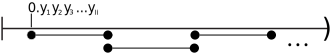
\includegraphics[width=0.5\textwidth]{images/kraftintervals2.pdf}
	  \label{fig:kraftintervals}
	  \end{figure}
  \end{itemize}
  \proofbreak
  \vspace{-0.2cm}
  \begin{itemize}
  \item O intervalo da palavra $y_1 y_2 \ldots y_{l_i}$ corresponde ao conjunto de todos números que iniciam-se com
	$y_1 y_2 \ldots y_{l_i}$, e desta forma é um subintervalo do intervalo unitário.
  \item Além disso, $y_1 y_2 \ldots y_{l_i}$ não é prefixo para nenhuma outra palavra, desta forma os intervalos
	serão disjuntos.
  \item O tamanho do intervalo associado à palavra $y_1 y_2 \ldots y_{l_i}$ é $D^{-l_i}$.
  \item Como todos intervalos estão dentro do intervalo $[0,1)$ teremos que
	\begin{equation}
	\sum_i D^{-l_i} \leq 1
	\end{equation}
  \vspace{-0.2cm}
  \item A prova da proposição inversa é similar ao caso finito.
  \end{itemize}
  \end{proof}
\end{frame}


\subsection{Código Ótimo}
\begin{frame}[allowframebreaks]
  \frametitle{Em busca de um código ótimo}
  \begin{itemize}
  \item Código de prefixo $\Leftrightarrow$ desigualdade de Kraft.
  \item Precisamos encontrar os comprimentos $l_i$ que satisfazem Kraft para obter um código de prefixo.
  \item Objetivo: encontrar um código de prefixo com o comprimento esperado mínimo.
	\begin{equation}
	L(C) = \sum_{i} p_i l_i
	\end{equation}
  \item Temos então um problema de otimização com restrição:
	encontrar
	\begin{equation}
	\min_{\{l_{1:m}\} \in \mathbb{Z}_{+}^m} \sum_i p_i l_i
	\end{equation}
	sujeito a
	\begin{equation}
	\sum_i D^{-l_i} \leq 1
	\end{equation}
  \item Temos um problema de programação em inteiros que é um problema NP-difícil. Este problema
	não provável de ser solucionado eficientemente (a menos que $P=NP$). 
  \item Vamos relaxar a condição de que $l_i$ precisa ser inteiro e considerar o Lagrangiano
	\begin{equation}
	J = \sum_i p_i l_i + \lambda \left( \sum_i D^{-l_i} - 1 \right)
	\end{equation}
  \item Tomando as derivadas e igualando a zero, teremos:
	\begin{eqnarray}
	\frac{\partial J}{\partial l_i} = p_i - \lambda D^{-l_i} \ln D = 0 \nonumber \\
	\Rightarrow D^{-l_i} = \frac{p_i}{\lambda \ln D}
	\end{eqnarray}
  	\begin{equation}
	\frac{\partial J}{\partial \lambda} = \sum_i D^{-l_i} - 1 = 0 \Rightarrow \lambda = 1 / \ln D
	\end{equation}
	\begin{equation}
	\Rightarrow D^{-l_i} = p_i \quad \text{implicando em} \quad l^\ast_i = -\log_D p_i
        \end{equation}
  \item Isto implica que
	\begin{equation}
	L^\ast = \sum_i p_i l_i^\ast = - \sum_i p_i \log_D p_i = H_D (X) = H(X) / \log D
	\end{equation}
  \item Os comprimentos ótimos para as palavras de um código são, de acordo com a otimização realizada,
	dados pela entropia, assumindo que seja possível utilizar comprimentos fracionários.
  \item Como $l^\ast_i = - \log_D p_i$, isto implica que os ``comprimentos'' ótimos (mesmo que fracionários)
	são iguais à informação do evento. I.e., o menor comprimento para codificação é inerentemente a informação
	sobre este evento (princípio da descrição mínima - Navalha de Occam).
  \item Com a codificação em blocos podemos aproximar do limite ótimo em que os comprimentos dos códigos por símbolos
	são valores fracionários.
  \end{itemize}
\end{frame}
\note{
\textbf{NP-Difícil}

``Um problema H é NP-difícil se e somente se (sse) existe um problema NP-completo L 
que é Turing-redutível em tempo polinomial para H (i.e., L?=?TH). Em outras palavras, 
L pode ser resolvido em tempo polinomial por uma Máquina de Turing não determinística 
com um oráculo para H. Informalmente, podemos pensar em um algoritmo que pode chamar 
tal Máquina de Turing Não-Determinística como uma sub-rotina para resolver H, e resolver L 
em tempo polinomial, se a chamada da sub-rotina leva apenas um passo para computar. 
Problemas NP-difíceis podem ser de qualquer tipo: problemas de decisão, problemas de 
pesquisa ou problemas de otimização.'' (Wikipedia)
}
\note{
``Em problemas de otimização, o método dos multiplicadores de Lagrange permite encontrar 
extremos (máximos e mínimos) de uma função de uma ou mais variáveis suscetíveis a uma ou mais restrições.

Por exemplo, considere o problema de otimização:
\begin{itemize}
\item maximize $f(x,y)$ ou seja, deseja-se encontrar o ponto máximo desta função
\item sujeito a $g(x,y) = c$.
\end{itemize}

    \begin{figure}[h!]
    \centering
    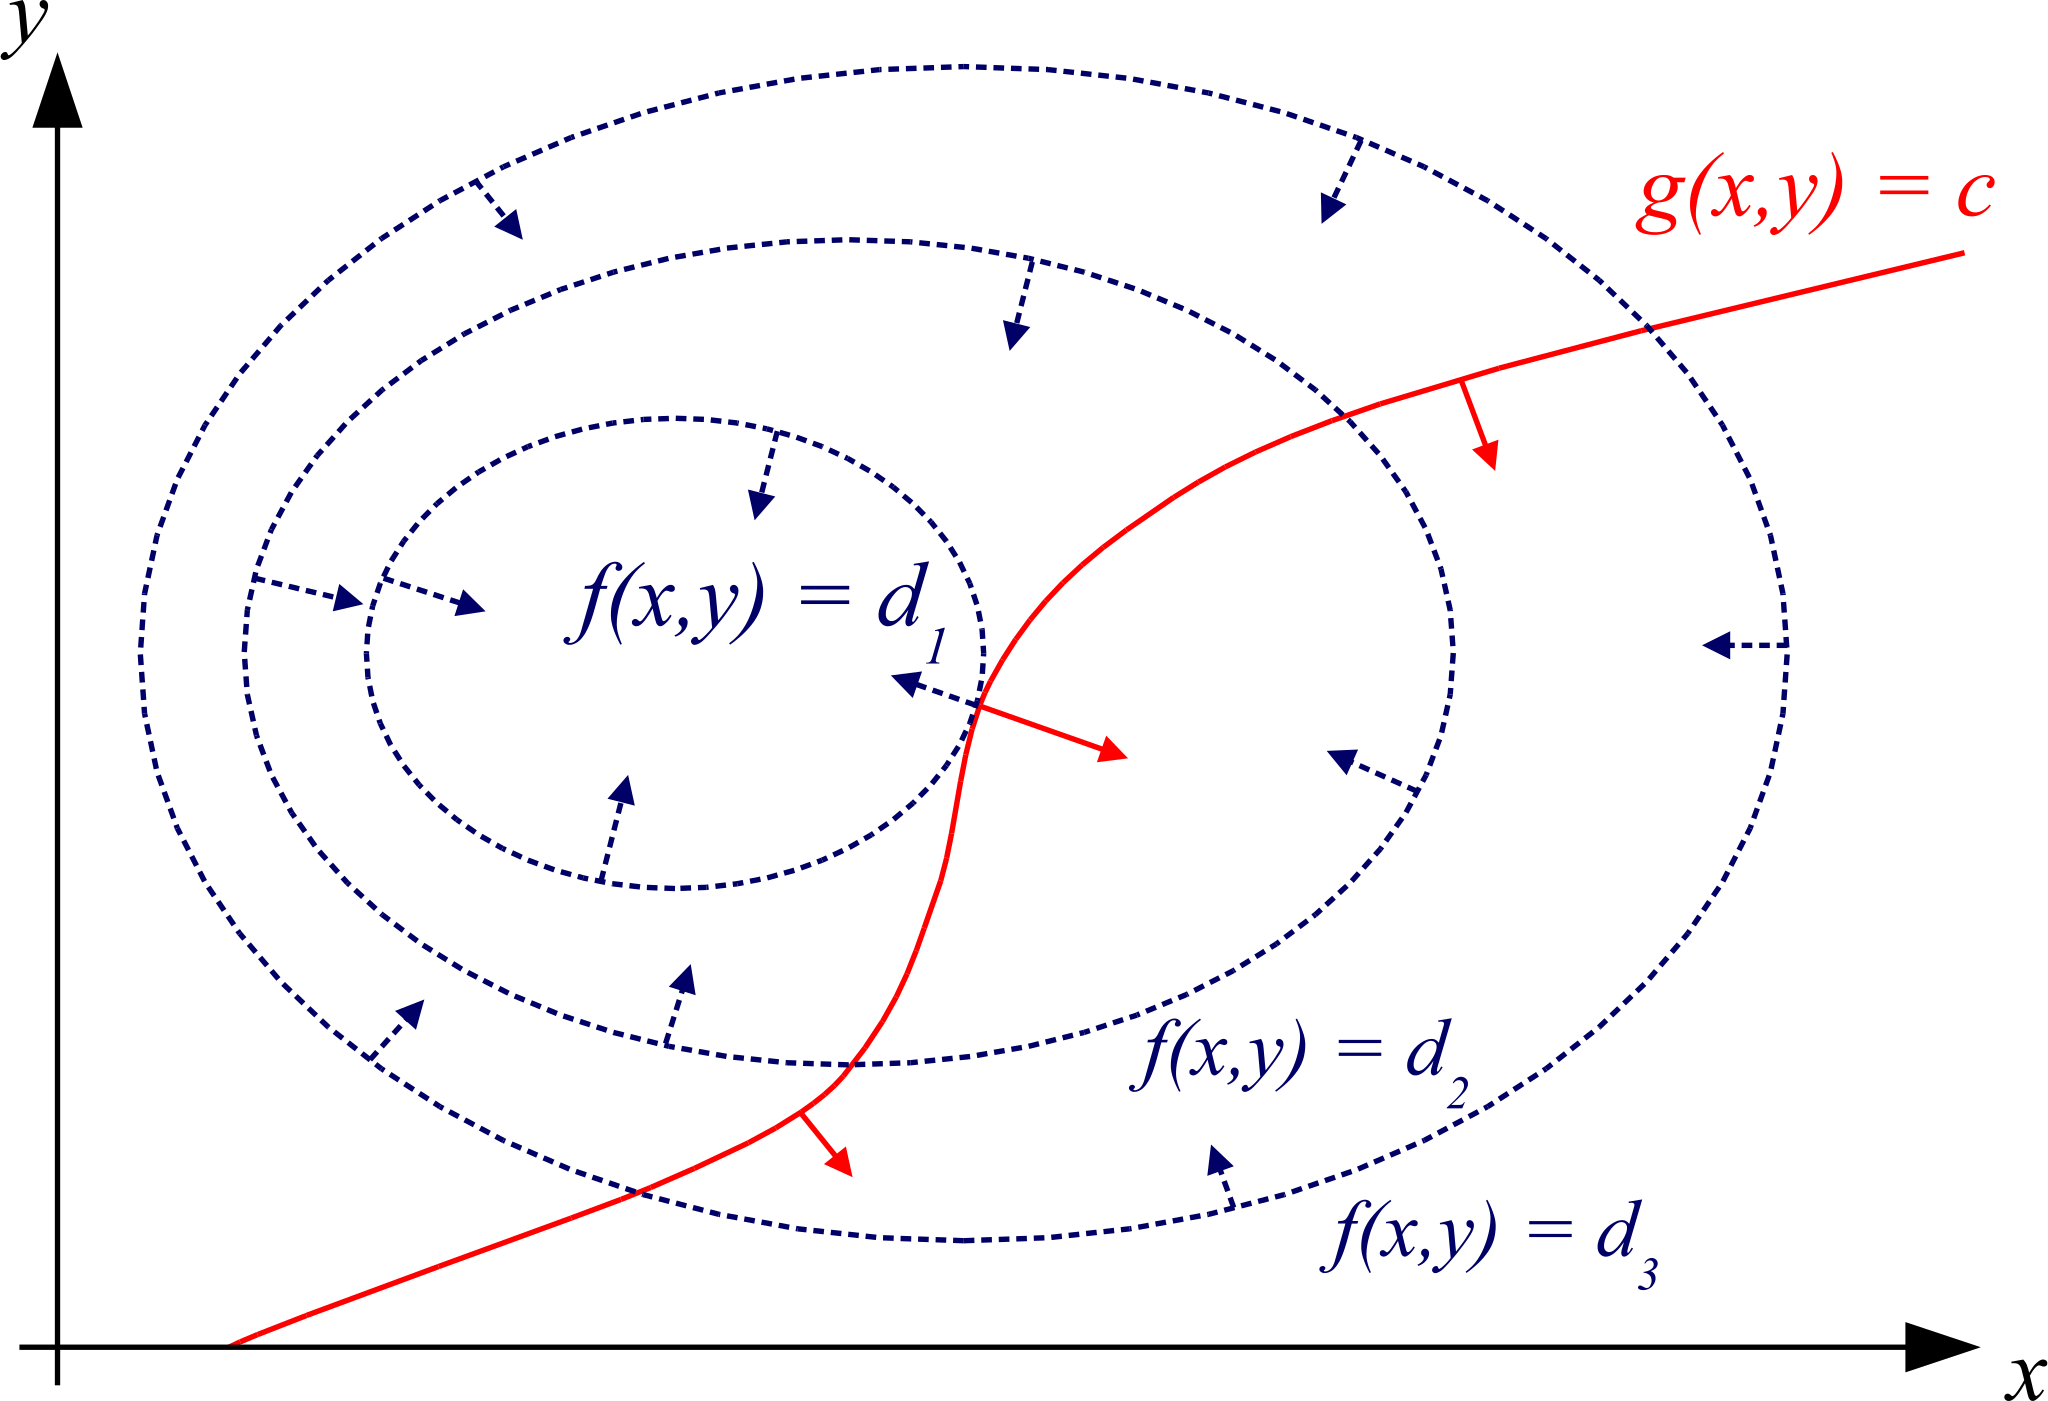
\includegraphics[width=0.4\textwidth]{images/LagrangeMultipliersEx2.pdf}
    \label{fig:LagrangeMultipliersEx}
    \end{figure}
}
\note{
O método consiste em introduzir uma variável nova ($\lambda$ normalmente), 
chamada de multiplicador de Lagrange. A partir disso, estuda-se a função de Lagrange, assim definida:
\begin{equation}
\Lambda(x,y,\lambda) = f(x,y) + \lambda \cdot \Big(g(x,y)-c\Big),
\end{equation}

Nesta função, o termo $\lambda$ pode ser adicionado ou subtraído. Se $f(x,y)$ é um ponto de máximo 
para o problema original, então existe um $\lambda$ tal que $(x,y,\lambda)$ é um ponto estacionário 
para a função lagrangiana, ou seja, existe um ponto para o qual as derivadas parciais de $\Lambda$
são iguais a zero.

No entanto, nem todos os pontos estacionários permitem uma solução para o problema original. 
Portanto, o método dos multiplicadores de Lagrange garante uma condição necessária para a 
otimização em problemas de otimização com restrição.'' (Wikipedia)
}
\note{
\textbf{Navalha de Occam}

``A Navalha de Occam ou Navalha de Ockham é um princípio lógico atribuído ao lógico 
e frade franciscano inglês Guilherme de Ockham (século XIV).

O princípio afirma que a explicação para qualquer fenómeno deve supor apenas as premissas 
estritamente necessárias à sua explicação e eliminar todas as que não causariam qualquer 
diferença aparente nas predições da hipótese ou teoria. O princípio é frequentemente designado 
pela expressão latina \textit{Lex Parsimoniae} (Lei da Parcimónia) enunciada como: 
\textit{``entia non sunt multiplicanda praeter necessitatem''} (as entidades não devem ser 
multiplicadas além da necessidade).

O princípio recomenda assim que se escolha a teoria explicativa que implique o menor número 
de premissas assumidas e o menor número de entidades.
}


\begin{frame}[allowframebreaks]
  \frametitle{Código Ótimo}
  \begin{theorem}
  Entropia é o comprimento esperado mínimo. O comprimento esperado $L$ de qualquer código
  $D$-ário instantâneo (satisfaz Kraft por conseguinte) para uma v.a. $X$ é tal que
	\begin{equation}
	L \geq H_D (X)
	\end{equation}
  com igualdade sse $D^{-l_i} = p_i$.
  \end{theorem}

  \framebreak

  \begin{proof}
  \begin{eqnarray}
  L - H_D (X) &=& \sum_i p_i l_i - \sum_i p_i \log_D 1/p_i \nonumber \\
		&=& - \sum_i p_i \log_D D^{-l_i} + \sum_i p_i \log_D p_i 
  \end{eqnarray}
  \proofbreak
  \begin{eqnarray}
  L - H_D (X) &=& \ldots \nonumber \\
		&=& - \sum_i p_i \log_D D^{-l_i} + \nonumber \\
		&& \underbrace{ \log_D \left( \sum_i D^{-l_i} \right) - \log_D \left( \sum_i D^{-l_i} \right)  }_{=0} + \nonumber \\
		&& \sum_i p_i \log_D p_i 
  \end{eqnarray}

  \proofbreak
  {\scriptsize (interlúdio)}
  \vspace{-0.6cm}
  \begin{eqnarray}
  - \sum_i p_i \log_D D^{-l_i} + \log_D \left( \sum_j D^{-l_j} \right) +  \sum_i p_i \log_D p_i = \nonumber \\
  - \sum_i p_i \log_D D^{-l_i} + \left( \underbrace{ \sum_i p_i }_{=1} \right) \log_D \left( \sum_i D^{-l_i} \right) + \sum_i p_i \log_D p_i = \nonumber \\
  - \sum_i p_i \log_D D^{-l_i} + \sum_i p_i \log_D \left( \sum_j D^{-l_j} \right) + \sum_i p_i \log_D p_i = \ldots
  \end{eqnarray}
  \proofbreak
  \begin{eqnarray}
  \ldots &=&  \sum_i p_i \log_D \frac{p_i \left( \sum_j D^{-l_j} \right)}{D^{-l_i}} \nonumber \\
   	&=&  \sum_i p_i \log_D \frac{p_i}{\frac{D^{-l_i}}{\left( \sum_j D^{-l_j} \right)}} = \sum_i p_i \log_D \frac{p_i}{r_i}
  \end{eqnarray}
  onde definimos 
	\begin{equation}
	r_i = \frac{D^{-l_i}}{\sum_j D^{-l_j}} .
	\end{equation}
  \proofbreak
  Teremos assim
  \vspace{-0.3cm}
  \begin{eqnarray}
  L - H_D (X) &=& \ldots \nonumber \\
		&=& \sum_i p_i \log_D \frac{p_i}{r_i} - \log_D \left( \sum_i D^{-l_i} \right) \nonumber \\
		&=& \underbrace{D(p \mid\mid r)}_{ \geq 0} + \underbrace{\log_D (1/c)}_{ \geq 0} \nonumber \\
		&\geq& 0 \\
		&& \text{ já que } c \leq 1 \text{ pois satisfaz Kraft, } \nonumber \\
		&& \quad \quad \text{ onde } c = \sum_i D^{-l_i}. \nonumber
  \end{eqnarray}
  \end{proof}

  \begin{itemize}
  \item Mostramos que $L \geq H_D (X)$.
  \item A igualdade $L=H$ é alcançada sse $p_i = D^{-l_i}$ para todo $i$ sse $-\log_D p_i$ for um inteiro. Neste caso 
	teremos $c = \sum_i D^{-l_i} = 1$.
  \end{itemize}

  \begin{definition}[$D$-ádico]
  Uma distribuição probabilística é $D$-ádica com relação a $D$ se cada uma das probabilidades é da forma $D^{-n}$
  para algum $n$.
  \end{definition}
  \begin{itemize}
  \item Exemplo: Quando $D=2$, a distribuição $\left[ \frac{1}{2}, \frac{1}{4}, \frac{1}{8}, \frac{1}{8} \right] = [2^{-1}, 2^{-2}, 2^{-3}, 2^{-3}]$ é $2$-ádica.
  \item Teremos $L=H$ quando a distribuição for $D$-ádica.
  \end{itemize}
\end{frame}

\begin{frame}[allowframebreaks]
  \frametitle{Sumário}
  \begin{itemize}
  \item No problema de otimização relaxado, retiramos a restrição de que os comprimentos dos códigos
	precisam ser inteiros, desta forma obtivemos $E l = H$.
  \item Assumindo que Kraft seja satisfeito (existe um código de prefixo com tais comprimentos)
	teremos comprimentos inteiros de forma que $E l \geq H$. 
	\begin{itemize}
	\item Se ainda $l_i = -\log_D p_i$ é
	inteiro, para todo $i$, então teremos a igualdade $E l = H$. 
	\item Se $l_i \neq -\log_D p_i$, mas $l_i$ é inteiro, teremos estritamente $E l > H$.
	\end{itemize}
  \end{itemize}
\end{frame}


\subsection{Códigos de Shannon}
\begin{frame}[allowframebreaks]
  \frametitle{Como construir um código buscando o ótimo}
  \begin{itemize}
  \item Vimos anteriormente que o limite ótimo para o comprimento esperado do código é a entropia. Desta forma
	$L-H$ é uma medida do quão distante estamos deste ponto ótimo.
  \item $L-H = D(p \mid \mid r) + \log_D 1/c$, onde $c = \sum_i D^{-l_i}$ e $r_i = \frac{D^{-l_i}}{\sum_j D^{-l_j}}$.
  \item Para criar o código devemos buscar a distribuição $D$-ádica mais próxima (em termos de divergência de KL)
	da distribuição $p$ e então construir um código seguindo a proposição inversa de Kraft.
  \item De forma geral, a menos que $P=NP$, é difícil encontrar a distribuição $D$-ádica mais próxima (no sentido de KL)
	da distribuição $p$ (problema de programação linear).
  \end{itemize}
\end{frame}


\begin{frame}[allowframebreaks]
  \frametitle{Códigos de Shannon}
  \begin{itemize}
  \item Considerar o comprimento como inteiro mais próximo do valor ótimo: $l_i = \lceil \log_D 1/p_i \rceil$.
  \item Devemos verificar se esta escolha satisfaz Kraft:
	\begin{equation}
	\sum_i D^{-l_i} = \sum_i D ^{- \lceil \log_D 1/p_i \rceil} \leq \sum_i D^{-\log_D 1/p_i} = \sum_i p_i = 1
	\end{equation}
	Kraft é satisfeito, então existe um código de prefixo com estes comprimentos.
  \item Temos então os seguintes limites para os comprimentos:
	\begin{equation}
	\log_D \frac{1}{p_i} \leq l_i \leq \log_D \frac{1}{p_i} + 1
	\end{equation}
  \item Tomando o valor esperando teremos:
	\begin{eqnarray}
	E_p \left[ \log_D \frac{1}{p_i} \right]  & \leq E_p \left[ l_i \right] \leq E_p & \left[ \log_D \frac{1}{p_i} + 1 \right] \nonumber \\
	\sum_i p_i \log_D \frac{1}{p_i} & \leq L \leq & \sum_i p_i \left( \log_D \frac{1}{p_i} + 1 \right) \nonumber \\
	H_D(X) & \leq L \leq & H_D(X) + 1
	\end{eqnarray}
 	Ou seja, no máximo a 1 bit (ou $D$-it, bit se $D=2$) de distância da entropia.
  \item Além disso temos que $H \leq L^\ast \leq L$, onde $L^\ast$ é o comprimento ótimo para códigos de comprimento
	inteiro (obs.: é possível que os comprimentos ótimos inteiros não satisfaçam Kraft). 
  \end{itemize}
  
  \framebreak
  \begin{theorem}
  Sejam $l_1^\ast, l_2^\ast, \ldots, l_m^\ast$ comprimentos inteiros ótimos de códigos para uma fonte $p$ e um
  alfabeto $D$-ário. $L^\ast$ é o comprimento esperado. Então
	\begin{equation}
	H_D(X) \leq L^\ast \leq H_D(X) + 1
	\end{equation}
  \end{theorem}
  \begin{itemize}
  \item O custo adicional de utilizar inteiros (ao invés de valores fracionários) para os comprimentos das palavras
	não é maior do que um bit por símbolo.
  \item Este custo adicional é significativo? (muito ruim?) Depende de $H$.
  \item Definimos então a eficiência de um código:
  \end{itemize}
  
  \begin{definition}[Eficiência de um código]
  A eficiência de um código é definida da seguinte forma
	\begin{equation}
	0 \leq \text{eficiência} \triangleq \frac{H_D(X)}{E l(X)} \leq 1
	\end{equation}
  \end{definition}

  \begin{itemize}
  \item Se $E l(X) = H_D (X) + 1$, então a eficiência $\rightarrow 1$ quando $H(X) \rightarrow \infty$.
  \item Eficiência $\rightarrow 0$ quando $H(X) \rightarrow 0$.
  \item A entropia precisa ser muito grande para que a tenhamos uma boa eficiência.
  \item Para alfabetos pequenos é impossível ter boa eficiência. Por exemplo: $\mathcal{D} = \{0,1\}$, então
	$\max H(X) = 1$, desta forma a melhor eficiência possível é 50\%.
  \end{itemize}
\end{frame}


\begin{frame}[allowframebreaks]
  \frametitle{Melhorando a eficiência}
  \begin{itemize}
  \item O código visto anteriormente é inerentemente desvantajoso, a menos que a distribuição seja $D$-ádica.
  \item Podemos melhorar a eficiência codificando mais de um símbolo por vez (codificação em bloco). Isto
	equivale a aumentar o alfabeto e aumentar a entropia.
  \item Vamos chamar de $L_n$ o comprimento esperado por símbolo de uma sequência de $n$ símbolos $x_{1:n}$.
	\begin{equation}
	L_n = \frac{1}{n} \sum_{x_{1:n} \in \mathcal{X}^n} p(x_{1:n}) l(x_{1:n}) = \frac{1}{n} E l(x_{1:n})
	\end{equation}
  \item Utilizando os comprimentos do código de Shannon, teremos
	\begin{eqnarray}
	\log 1/p_i & \leq l_i \leq & \log 1/p_i + 1 \nonumber \\
	\sum_i p_i \log 1/p_i & \leq \sum_i p_i l_i \leq & \sum_i p_i \left( \log 1/p_i + 1 \right) \nonumber \\
	H(X_1,\ldots,X_n) & \leq E l(X_{1:n}) \leq & H(X_1,\ldots,X_n) + 1
	\end{eqnarray}
  \item Se $X_i$ são i.i.d., então $H(X_1,\ldots,X_n) = nH(X_i)$.
  \item Teremos assim
	\begin{equation}
	H(X) \leq L_n \leq H(X) + \frac{1}{n}
	\end{equation}
  \item Quando $n$ cresce, a penalidade por símbolo imposta ao código de Shannon diminui e 
	conseguiremos assim aproximar-nos do limite da Entropia (por símbolo), embora teremos que
	mais uma vez adotar a estratégia de codificação em blocos.
  \end{itemize}
\end{frame}

\begin{frame}[allowframebreaks]
  \frametitle{Processos Estocásticos}
  \begin{itemize}
  \item Considere um processo estocástico estacionário (ergódico), então
	\begin{eqnarray}
	H(X_1,\ldots,X_n) & \leq E l(X_{1:n}) \leq & H(X_1,\ldots,X_n) + 1 \nonumber \\
	\frac{ H(X_1,\ldots,X_n) }{n} & \leq L_n \leq & \frac{ H(X_1,\ldots,X_n) }{n} + \frac{1}{n}
	\end{eqnarray}
  \item Se o processo é estacionário, então $L_n \rightarrow H(\mathcal{X})$ (taxa de entropia) quando $n \rightarrow \infty$.
  \end{itemize}
  \begin{theorem}
  O comprimento mínimo esperado de código por símbolo satisfaz
	\begin{equation}
	\frac{ H(X_1,\ldots,X_n) }{n} \leq L_n^\ast \leq \frac{ H(X_1,\ldots,X_n) }{n} + \frac{1}{n}
	\end{equation}
  se $X_i$ é estacionário. Então $ L_n^\ast \rightarrow H(\mathcal{X})$.
  \end{theorem}
\end{frame}

\begin{frame}[allowframebreaks]
  \frametitle{Codificando para a distribuição errada.}
  \begin{itemize}
  \item Em geral a distribuição subjacente não é conhecida. Isto implica que existem erros nos cálculos.
  \item O código de Shannon utiliza $l(x) = \lceil \log 1/q(x) \rceil$, mas a real distribuição é
	$p(x) \neq q(x)$. O que implica essa diferença?
  \item Vamos recalcular o valor esperado do comprimento do código, agora utilizando esta informação.
	\begin{eqnarray}
	E l(X) &=& \sum_x p(x) \lceil \log 1/q(x) \rceil \leq \sum_x p(x) \left( \log \frac{1}{q(x)} + 1 \right) \nonumber \\
		&=& \sum_x p(x) \left( \log \frac{p(x)}{q(x)} \frac{1}{p(x)} + 1 \right) \nonumber \\
		&=& \sum_x p(x) \log \frac{p(x)}{q(x)} + \sum_x p(x) \log \frac{1}{p(x)} + 1 \nonumber \\
		&=& D(p \mid \mid q) + H(p) + 1
	\end{eqnarray}
  \item $D(p \mid \mid q)$ é o custo adicional por símbolo causado por utilizar a distribuição errada.
  \end{itemize}
  
  \begin{theorem}
  O comprimento esperado de um código sob a distribuição $p(x)$ com $l(x) = \lceil \log 1/q(x) \rceil$ satisfaz
	\begin{equation}
	H(p) + D(p \mid \mid q) \leq E_p l(X) \leq H(p) + D(p \mid \mid q) + 1
	\end{equation}
  \end{theorem}
  \begin{itemize}
  \item No melhor caso estaremos sofrendo uma penalidade de $D(p \mid \mid q)$.
  \end{itemize}
\end{frame}


\subsection{Kraft revisitado}
\begin{frame}[allowframebreaks]
  \frametitle{Kraft revisitado}
  \begin{itemize}
  \item O objetivo é encontrar um código unívoco (unicamente decodificável) com comprimento esperado de palavra mínimo.
  \item Observando as classes de códigos, podemos imaginar que a classe mais ampla é a mais provável de se encontrar tal código desejado.
  \end{itemize}

  \begin{figure}[h!]
  \centering
  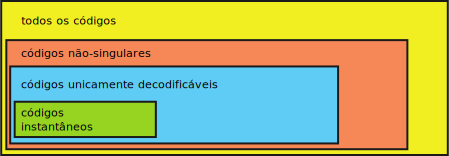
\includegraphics[width=0.5\textwidth]{images/tiposcodigos.pdf}
  \label{fig:tiposcodigosagain}
  \end{figure}

  \begin{itemize}
  \item Kraft é verdadeiro para códigos instantâneos (e vice-versa).
  \item Dentre os códigos unicamente decodificáveis, podemos encontrar um código melhor (menor comprimento esperado)
	do que um código de prefixo? (Já que estamos analisando uma classe maior de código).
  \end{itemize}
 
  \begin{theorem}
  O comprimento de palavras de qualquer código unicamente decodificável (não necessariamente instantâneo)
  deve satisfazer a desigualdade de Kraft $\sum_i D^{-l_i} \leq 1$. Por outro lado, dado um conjunto de comprimentos
  que satisfazem Kraft, é possível construir um código unicamente decodificável.
  \end{theorem}
  \begin{proof}
  A proposição inversa já foi previamente mostrada, uma vez que mostramos como construir um código instantâneo 
  utilizando um conjunto de comprimentos satisfazendo Kraft.
  \end{proof}

  \framebreak
  Antes de provar o teorema vamos mostrar o seguinte Lemma.
  \begin{lemma}
  Seja $\mathcal{X} = \{x_1, x_2, \ldots, x_m \}$, $\vert \mathcal{X} \vert = m$, temos o seguinte

  \begin{eqnarray}
  \left( \sum_{x \in \mathcal{X}} D^{-l(x)} \right)^k &=& \left( \sum_{i=1}^{m} D^{-l(x_i)} \right)^k \nonumber \\
		&=& \left( D^{-l(x_1)} + D^{-l(x_2)} + \ldots + D^{-l(x_m)}  \right)^k \nonumber \\
		&=& \sum_{\substack{ n_1, n_2, \ldots, n_m \geq 0 \\ n_1 + n_2 + \ldots + n_m = k}} 
			\frac{k!}{n_1! n_2! \ldots n_m!} D^{-l(x_1)n_1} \ldots D^{-l(x_m)n_m} \nonumber
  \end{eqnarray}
  \lemmabreak

  Cada termo no somatório acima é devido a uma sequência de comprimento $k$ formada pela combinação dos símbolos
  em $\mathcal{X}$. 

  Podemos interpretar a série como 
  \begin{equation}
  \left( \sum_{x \in \mathcal{X}} D^{-l(x)} \right)^k = \sum_{x_{1:k} \in \mathcal{X}^k} D^{-l(x_1)} D^{-l(x_2)} \ldots D^{-l(x_k)} 
  \end{equation}
  \end{lemma}

  \framebreak
  \begin{proof}
  \begin{itemize}
  \item Dado um código unicamente decodificável (não necessariamente instantâneo) com comprimentos $l(x)$
	e com extensão com comprimentos dados por $l(x_1, \ldots, x_k) = \sum_{i=1}^k l(x_i)$, queremos mostrar
	que $\sum_x D^{-l(x)} \leq 1$.
  \end{itemize}
  \proofbreak
  \begin{itemize}
  \item Vamos definir $S = \sum_{x \in \mathcal{X}} D^{-l(x)}$ e então
  \end{itemize}
  \begin{eqnarray}
	S^k &=& \left( \sum_{x \in \mathcal{X}} D^{-l(x)} \right)^k \nonumber \\
		&=& \sum_{x_{1:k} \in \mathcal{X}^k} D^{-l(x_1)} D^{-l(x_2)} \ldots D^{-l(x_k)} \nonumber \\
			&& \text{(veja lemma)} \nonumber \\
		&=& \sum_{x_{1:k} \in \mathcal{X}^k} D^{- \left( \sum_{i=1}^k l(x_i) \right)} 
  \end{eqnarray}
  \proofbreak
  \vspace{-0.5cm}
  \begin{eqnarray}
        S^k &=& \ldots \\
		&=& \sum_{x_{1:k} \in \mathcal{X}^k} D^{-l(x_{1:k})} \nonumber \\
		&=& \sum_{m=1}^{k l_{\text{max}}} a(m) D^{-m}
  \end{eqnarray}
  onde $l_{\text{max}} = \max_x l(x)$, $a(m)$ é o número de sequências $x_{1:k}$ mapeadas em palavras de comprimento $m$,
  i.e.,
  \begin{equation}
	a(m) = \left\vert \{ x_{1:k} \in \mathcal{X}^k : l(x_{1:k}) = m \} \right\vert
  \end{equation}
  \proofbreak
  Existem $D^m$ palavras de comprimento $m$, e cada uma delas pode ter no máximo uma sequência da fonte associada,
  já que o código é unicamente decodificável. Então $a(m) \leq D^m$, e assim
  \begin{eqnarray}
  \underbrace{S^k}_{\text{exponencial em } k} &=& \sum_{m=1}^{k l_{\text{max}}} a(m) D^{-m} \nonumber \\
		&\leq& \sum_{m=1}^{k l_{\text{max}}} D^m D^{-m} = \underbrace{k l_{\text{max}}}_{\text{polinomial em } k} \quad \forall k
  \end{eqnarray}
  Isto só pode ser verdade para todo $k$ se $S \leq 1$. 
  \proofbreak
  Teremos então
  \begin{equation}
  S = \sum_{x \in \mathcal{X}} D^{-l(x)} \leq 1 .
  \end{equation}
  \end{proof}
  
  Código unicamente decodificável vs Código Instantâneo
  \begin{itemize}
  \item Todo código instantâneo é unicamente decodificável.
  \item Todos códigos unicamente decodificável devem satisfazer Kraft.
  \item Então podemos utilizar os mesmos comprimentos de palavras e construir um código de prefixo.
  \item Conclusão: não faz sentido utilizar a classe mais ampla de código unicamente decodificáveis, 
	é melhor utilizar um código de prefixo, que terá o mesmo comprimento esperado e será
	instantâneo.
  \end{itemize}
\end{frame}

\subsection{Algoritmo de Sardinas-Patterson}
\begin{frame}[allowframebreaks]
  \frametitle{Algoritmo de Sardinas-Patterson}

  O algoritmo de Sardinas-Patterson fornece uma maneira de determinar, em tempo polinomial, 
  se um determinado código é unicamente decodificável ou não (ver exercício 5.27 do livro).


  \vspace{5em}
  Sardinas, August Albert; Patterson, George W. (1953), ``A necessary and sufficient condition
  for the unique decomposition of coded messages'', Convention Record of the I.R.E., 1953
  National Convention, Part 8: Information Theory, pp. 104-108.
\end{frame}

